% Options for packages loaded elsewhere
\PassOptionsToPackage{unicode}{hyperref}
\PassOptionsToPackage{hyphens}{url}
%
\documentclass[
]{article}
\usepackage{lmodern}
\usepackage{amssymb,amsmath}
\usepackage{ifxetex,ifluatex}
\ifnum 0\ifxetex 1\fi\ifluatex 1\fi=0 % if pdftex
  \usepackage[T1]{fontenc}
  \usepackage[utf8]{inputenc}
  \usepackage{textcomp} % provide euro and other symbols
\else % if luatex or xetex
  \usepackage{unicode-math}
  \defaultfontfeatures{Scale=MatchLowercase}
  \defaultfontfeatures[\rmfamily]{Ligatures=TeX,Scale=1}
\fi
% Use upquote if available, for straight quotes in verbatim environments
\IfFileExists{upquote.sty}{\usepackage{upquote}}{}
\IfFileExists{microtype.sty}{% use microtype if available
  \usepackage[]{microtype}
  \UseMicrotypeSet[protrusion]{basicmath} % disable protrusion for tt fonts
}{}
\makeatletter
\@ifundefined{KOMAClassName}{% if non-KOMA class
  \IfFileExists{parskip.sty}{%
    \usepackage{parskip}
  }{% else
    \setlength{\parindent}{0pt}
    \setlength{\parskip}{6pt plus 2pt minus 1pt}}
}{% if KOMA class
  \KOMAoptions{parskip=half}}
\makeatother
\usepackage{xcolor}
\IfFileExists{xurl.sty}{\usepackage{xurl}}{} % add URL line breaks if available
\IfFileExists{bookmark.sty}{\usepackage{bookmark}}{\usepackage{hyperref}}
\hypersetup{
  pdftitle={Climate variability indices for ecological and crop models in R: the climatrends package},
  hidelinks,
  pdfcreator={LaTeX via pandoc}}
\urlstyle{same} % disable monospaced font for URLs
\usepackage[margin=1in]{geometry}
\usepackage{color}
\usepackage{fancyvrb}
\newcommand{\VerbBar}{|}
\newcommand{\VERB}{\Verb[commandchars=\\\{\}]}
\DefineVerbatimEnvironment{Highlighting}{Verbatim}{commandchars=\\\{\}}
% Add ',fontsize=\small' for more characters per line
\usepackage{framed}
\definecolor{shadecolor}{RGB}{248,248,248}
\newenvironment{Shaded}{\begin{snugshade}}{\end{snugshade}}
\newcommand{\AlertTok}[1]{\textcolor[rgb]{0.94,0.16,0.16}{#1}}
\newcommand{\AnnotationTok}[1]{\textcolor[rgb]{0.56,0.35,0.01}{\textbf{\textit{#1}}}}
\newcommand{\AttributeTok}[1]{\textcolor[rgb]{0.77,0.63,0.00}{#1}}
\newcommand{\BaseNTok}[1]{\textcolor[rgb]{0.00,0.00,0.81}{#1}}
\newcommand{\BuiltInTok}[1]{#1}
\newcommand{\CharTok}[1]{\textcolor[rgb]{0.31,0.60,0.02}{#1}}
\newcommand{\CommentTok}[1]{\textcolor[rgb]{0.56,0.35,0.01}{\textit{#1}}}
\newcommand{\CommentVarTok}[1]{\textcolor[rgb]{0.56,0.35,0.01}{\textbf{\textit{#1}}}}
\newcommand{\ConstantTok}[1]{\textcolor[rgb]{0.00,0.00,0.00}{#1}}
\newcommand{\ControlFlowTok}[1]{\textcolor[rgb]{0.13,0.29,0.53}{\textbf{#1}}}
\newcommand{\DataTypeTok}[1]{\textcolor[rgb]{0.13,0.29,0.53}{#1}}
\newcommand{\DecValTok}[1]{\textcolor[rgb]{0.00,0.00,0.81}{#1}}
\newcommand{\DocumentationTok}[1]{\textcolor[rgb]{0.56,0.35,0.01}{\textbf{\textit{#1}}}}
\newcommand{\ErrorTok}[1]{\textcolor[rgb]{0.64,0.00,0.00}{\textbf{#1}}}
\newcommand{\ExtensionTok}[1]{#1}
\newcommand{\FloatTok}[1]{\textcolor[rgb]{0.00,0.00,0.81}{#1}}
\newcommand{\FunctionTok}[1]{\textcolor[rgb]{0.00,0.00,0.00}{#1}}
\newcommand{\ImportTok}[1]{#1}
\newcommand{\InformationTok}[1]{\textcolor[rgb]{0.56,0.35,0.01}{\textbf{\textit{#1}}}}
\newcommand{\KeywordTok}[1]{\textcolor[rgb]{0.13,0.29,0.53}{\textbf{#1}}}
\newcommand{\NormalTok}[1]{#1}
\newcommand{\OperatorTok}[1]{\textcolor[rgb]{0.81,0.36,0.00}{\textbf{#1}}}
\newcommand{\OtherTok}[1]{\textcolor[rgb]{0.56,0.35,0.01}{#1}}
\newcommand{\PreprocessorTok}[1]{\textcolor[rgb]{0.56,0.35,0.01}{\textit{#1}}}
\newcommand{\RegionMarkerTok}[1]{#1}
\newcommand{\SpecialCharTok}[1]{\textcolor[rgb]{0.00,0.00,0.00}{#1}}
\newcommand{\SpecialStringTok}[1]{\textcolor[rgb]{0.31,0.60,0.02}{#1}}
\newcommand{\StringTok}[1]{\textcolor[rgb]{0.31,0.60,0.02}{#1}}
\newcommand{\VariableTok}[1]{\textcolor[rgb]{0.00,0.00,0.00}{#1}}
\newcommand{\VerbatimStringTok}[1]{\textcolor[rgb]{0.31,0.60,0.02}{#1}}
\newcommand{\WarningTok}[1]{\textcolor[rgb]{0.56,0.35,0.01}{\textbf{\textit{#1}}}}
\usepackage{graphicx}
\makeatletter
\def\maxwidth{\ifdim\Gin@nat@width>\linewidth\linewidth\else\Gin@nat@width\fi}
\def\maxheight{\ifdim\Gin@nat@height>\textheight\textheight\else\Gin@nat@height\fi}
\makeatother
% Scale images if necessary, so that they will not overflow the page
% margins by default, and it is still possible to overwrite the defaults
% using explicit options in \includegraphics[width, height, ...]{}
\setkeys{Gin}{width=\maxwidth,height=\maxheight,keepaspectratio}
% Set default figure placement to htbp
\makeatletter
\def\fps@figure{htbp}
\makeatother
\setlength{\emergencystretch}{3em} % prevent overfull lines
\providecommand{\tightlist}{%
  \setlength{\itemsep}{0pt}\setlength{\parskip}{0pt}}
\setcounter{secnumdepth}{-\maxdimen} % remove section numbering
\usepackage{caption} \captionsetup[figure]{labelformat=empty}
\usepackage{booktabs}
\usepackage{longtable}
\usepackage{array}
\usepackage{multirow}
\usepackage{wrapfig}
\usepackage{float}
\usepackage{colortbl}
\usepackage{pdflscape}
\usepackage{tabu}
\usepackage{threeparttable}
\usepackage{threeparttablex}
\usepackage[normalem]{ulem}
\usepackage{makecell}
\usepackage{xcolor}
\newlength{\cslhangindent}
\setlength{\cslhangindent}{1.5em}
\newenvironment{cslreferences}%
  {\setlength{\parindent}{0pt}%
  \everypar{\setlength{\hangindent}{\cslhangindent}}\ignorespaces}%
  {\par}

\title{Climate variability indices for ecological and crop models in R:
the \texttt{climatrends} package}
\author{}
\date{\vspace{-2.5em}25 May 2020}

\begin{document}
\maketitle

\begin{quote}
Kauê de Sousa\textsuperscript{1,2{[}*{]}}, Jacob van
Etten\textsuperscript{2}, Svein Øivind Solberg\textsuperscript{1}\\
\textsuperscript{1} Department of Agricultural Sciences, Inland Norway
University of Applied Sciences, 2318 Hamar, Norway\\
\textsuperscript{2} Bioversity International, 00054 Maccarese, Rome,
Italy\\
\textsuperscript{{[}*{]}}Correspondence should be addressed to:
\href{mailto:kaue.desousa@inn.no}{\nolinkurl{kaue.desousa@inn.no}}
\end{quote}

\hfill\break

\hypertarget{introduction}{%
\section{Introduction}\label{introduction}}

Abiotic factors plays an important role in most ecological and crop
systems that depends on certain levels of temperature, light and
precipitation (and their interplay) to initiate important physiological
events (Schulze et al., 2019). In the walk of climate change, understand
how these factors drives the physiological processes is a key approach
to provide recommendations for adaptation and biodiversity conservation.

{[}\ldots continue\ldots{]}

\texttt{climatrends} aims to provide the R (R Core Team, 2020) toolkit
to compute extreme precipitation and temperature indices that serves as
input for climate and crop models (Kehel, Crossa, \& Reynolds, 2016; van
Etten et al., 2019), trends in climate change (Aguilar et al., 2005; de
Sousa et al., 2018) and applied ecology (Prentice et al., 1992; Liu \&
El-Kassaby, 2018).

{[}\ldots continue\ldots{]}

\hypertarget{methods-and-features}{%
\section{Methods and features}\label{methods-and-features}}

\hypertarget{implementation}{%
\subsection{Implementation}\label{implementation}}

Six main functions are provided, \texttt{crop\_sensitive()},
\texttt{ETo()}, \texttt{GDD()}, \texttt{late\_frost()},
\texttt{rainfall()} and \texttt{temperature()} with a default method for
numeric `vector's and additional methods implemented via the package
\texttt{methods} (R Core Team, 2020) for classes 'matrix' (or array),
`data.frame', and `sf' (of geometry POINT or POLYGON) (Pebesma, 2018).
The later two are designed to fetch data from cloud sources.

{[}\ldots continue\ldots{]}

say that the idea for the functions started with citizen science
projects that is why \texttt{day.one} and \texttt{span} may be variable
across locations. For time series analysis where fixed periods are
defined across many locations the indices can be adjusted with last.day.

{[}\ldots continue\ldots{]}

\hypertarget{temperature-and-precipitation-indices}{%
\subsection{Temperature and precipitation
indices}\label{temperature-and-precipitation-indices}}

Some explanation on the \texttt{temperature()} and \texttt{rainfall()}
functions.

\hypertarget{growing-degree-days}{%
\subsection{Growing degree-days}\label{growing-degree-days}}

Growing degree-days (gdd) is an heuristic tool in phenology that
measures heat accumulation and is used to predict plant and animal
development rates (Prentice et al., 1992). Growing degree-days are
calculated by taking the integral of warmth above a base temperature
(\(T_{0}\)). The function \texttt{GDD()} applies by default the
following equation.

Equation {[}1{]}

\[GDD = \frac{T_{max} + T_{min}}{2} - T_{0}\]

Where \(T_{max}\) is the maximum temperature in the given day,
\(T_{min}\) is the minimum temperature in the given day and \(T_{0}\) is
the minimum temperature for growth (as per the physiology of the focal
organism or ecosystem averages).

Additionally, the function \texttt{GDD()} offers three modified
equations designed for cold environments and for tropical environments.
For cold environments, where \(T_{min}\) may be lower than \(T_{0}\),
there are two modified equations that adjusts either \(T_{mean}\)
(variant a) or \(T_{min}\) (variant b). The variant a changes
\(T_{mean}\) to \(T_{0}\) if \(T_{mean} < T_{0}\) and is expressed as
follows.

Equation {[}2{]}

\[ GDD = max \left(\frac{T_{max} + T_{min}}{2} - T_{0}, \; 0 \right)\]

The variant b, is calculated using Equation 1, but adjusts \(T_{min}\)
or \(T_{max}\) to \(T_{0}\) if \(T < T_{0}\), the equation is adjusted
as follows.

Equation {[}3{]}

\[ T < T_{0} \; \rightarrow \; T = T_{0} \]

Where \(T\) may refer to \(T_{min}\) and/or \(T_{max}\) when the
condition of being below \(T_{0}\) applies.

For tropical areas, where the temperature may surpass a maximum
threshold (\(T_{0^{max}}\)), resulting in limited development, the
minimum temperature is adjusted using Equation 3 and the maximum
temperature is adjusted to a maximum base temperature as follow.

Equation {[}4{]}

\[ T_{max} > T_{0^{max}} \; \rightarrow \; T_{max} = T_{0^{max}} \]

Where \(T_{0^{max}}\) is the maximum base temperature for growth,
defined in \texttt{GDD()} using the argument \texttt{tbase\_max}.

These modified equations are defined as `a', `b' and `c', respectively,
and can be selected using the argument \texttt{equation}.

By default, the function returns the degree-days that is accumulated
over the time series using Equation 1. Additionally, the function may
return the daily values of degree-days or the number of days that a
given organism required to reach a certain number of accumulated
degree-days. These values are defined by `acc', `daily' or `ndays' and
can be adjusted using the argument \texttt{return.as}. The required
accumulated gdd is defined with argument \texttt{degree.days}. For
example, the Korean pine (\emph{Pinus koraiensis}) requires 105
\(^\circ C\) accumulated gdd to onset the photosynthesis (Wu, Guan,
Yuan, Wang, \& Jin, 2013). In that case, \texttt{GDD()} will calculate
the growing degree-days (\(gdd\)) and sum up the values until it reaches
105 \(^\circ C\) and return the number of days required in the given
season (\(GDD_{r}\)), as follows.

Equation {[}5{]}

\[\parallel GDD_{r} \parallel \: = \; ggd_1 \;+ \; ...  \; +  \; gdd_n\]

\hypertarget{late-spring-frost}{%
\subsection{Late-spring frost}\label{late-spring-frost}}

Explain how the \texttt{late\_frost()} is implemented.

\hypertarget{crop-related-indices}{%
\subsection{Crop-related indices}\label{crop-related-indices}}

Two functions in \textbf{climatrends} are mainly designed to capture the
effects of climate on the development and stress of crop species,
\texttt{crop\_sensitive} computes indices that aims to capture the
changes in temperature extremes during key phenological stages
(e.g.~anthesis), and \texttt{ETo()} computes the reference
evapotranspiration.

The reference evapotranspiration measures the influence of the climate
on a given organism water needs, generally a crop species (Brouwer \&
Heibloem, 1986). The function \texttt{ETo()} applies the Blaney-Criddle
method, a general theoretical method used when only air-temperature is
available locally. It should be noted that this method is not very
accurate and aims to provide the order of magnitude of
evapotranspitation. The reference evapotranspiration is calculated using
the following equation.

Equation {[}6{]}

\[ETo = p \times \left(0.46 \times \frac{T_{max} + T_{min}}{2} + 8 \right) \times K_c\]

Where \(p\) is the mean daily percentage of annual daytime hours,
\(T_{max}\) is the maximum temperature, \(T_{min}\) is the minimum
temperature, and \(K_c\) is the factor for organism water need.

The percentage of daytime hours (\(p\)) is calculated internally by the
`data.frame' and `sf' methods in \texttt{ETo()} using the given latitude
(taken from the inputted \texttt{object}) and date (taken from the
inputted \texttt{day.one}). It matches the latitude and date with a
table of daylight percentage derived from Brouwer and Heibloem (1986).
The table can be verified using \texttt{climatrends:::daylight}.

\hypertarget{examples}{%
\section{Examples}\label{examples}}

\hypertarget{some-gdd-related-analysis}{%
\subsection{Some GDD related analysis}\label{some-gdd-related-analysis}}

Use the data from seed germination or crop growth to compute GDD. Maybe
some GDD analysis in Scandinavia with data from the reindeer project.

\hypertarget{common-beans}{%
\subsection{Common beans}\label{common-beans}}

During five growing seasons (from 2015 to 2017 in Nicaragua), van Etten
et al.~(2019) conducted a crowdsourcing citizen-science trial testing 11
common beans varieties (\emph{Phaseolus vulgaris} L.) in 842
farmer-managed experimental plots. Sets of three varieties were
allocated randomly to farms as incomplete blocks. A Plackett--Luce model
was used to analyse the data, this model estimates for each variety the
probability that it wins, beating all other varieties in the set
(Turner, van Etten, Firth, \& Kosmidis, 2020). An earlier version of
\texttt{climatrends} was used in this research to capture the seasonal
climate variation, here we reproduce part of this analysis regarding
calculation and application of the climate indices. The approach here is
slightly different because if considers the growing-degree days from
planting date to maturity (the earlier study used planting date to the
end of reproductive stage) and add new indices to illustrate the package
implementation.

The data used here is available as supplementary materials
(\textbf{zenodo ref}) as \texttt{cbean}. This contains a data.frame with
a Plackett-Luce grouped rankings, the geographical coordinates of each
sampled plot and the planting dates from where each farmer decided to
start the experiment. The dates can differ from each other in the same
season. The temperature data used was the land surface temperature MODIS
(MYD11A2) (Wan, Hook, \& Hulley, 2015) and is storaged as an array with
two layers (1st for the day and 2nd for the night temperatures). Each
column corresponds to the dates (from 2015-09-10 to 2017-06-09) and the
rows corresponds to the rows in the \texttt{cbean} data.frame.

Since the phenological stages were not available, we estimate these
stages based on the amount of growing degree-days required to reach a
given stage using the function \texttt{GDD()}. For common beans, we
define 900 degree-days, from planting date to maturity (de Medeiros,
Daniel, \& Fengler, 2016). The input data is the array with the
temperature data, the vector with planting dates
(\texttt{cbean\$planting\_date}), the required amount of degree-days
passed to the argument \texttt{degree.days} and the character string
`ndays' specifying that the function must return the values as number of
days. \texttt{GDD()} calls internally the function
\texttt{get\_timeseries()} which will match the given dates in
\texttt{day.one} with the column names in the array and concatenate the
values for each row. Then \texttt{GDD()} computes the degree-days for
the time series and return the length of the vector where the
accumulated gdd reached the pre-defined threshold (900).

The degree-days spanned from 54 to 100 days as shown in Fig. 2a. For
simplicity we take the average per season and use this vector to compute
the temperature indices.

\begin{Shaded}
\begin{Highlighting}[]
\KeywordTok{library}\NormalTok{(}\StringTok{"climatrends"}\NormalTok{)}
\KeywordTok{library}\NormalTok{(}\StringTok{"PlackettLuce"}\NormalTok{)}
\KeywordTok{library}\NormalTok{(}\StringTok{"tidyverse"}\NormalTok{)}

\CommentTok{\# compute the number of days required to accumulate}
\CommentTok{\# gdd from planting date to maturity}
\NormalTok{gdd <{-}}\StringTok{ }\KeywordTok{GDD}\NormalTok{(modis, }
           \DataTypeTok{day.one =}\NormalTok{ cbean}\OperatorTok{$}\NormalTok{planting\_date, }
           \DataTypeTok{degree.days =} \DecValTok{900}\NormalTok{, }
           \DataTypeTok{return.as =} \StringTok{"ndays"}\NormalTok{)}

\CommentTok{\# add gdd to the cbean data and take the average }
\CommentTok{\# of gdd per season}
\NormalTok{cbean }\OperatorTok{\%<>\%}\StringTok{  }
\StringTok{  }\KeywordTok{mutate}\NormalTok{(}\DataTypeTok{gdd =}\NormalTok{ gdd}\OperatorTok{$}\NormalTok{gdd) }\OperatorTok{\%>\%}\StringTok{ }
\StringTok{  }\KeywordTok{group\_by}\NormalTok{(season) }\OperatorTok{\%>\%}\StringTok{ }
\StringTok{  }\KeywordTok{mutate}\NormalTok{(}\DataTypeTok{gdds =} \KeywordTok{as.integer}\NormalTok{(}\KeywordTok{mean}\NormalTok{(gdd)))}
\end{Highlighting}
\end{Shaded}

To compute the temperature indices we use the array with tempeture data,
the vector with planting dates, and the seasonal averaged degree-days
passed as a vector using the argument \texttt{span}.
\texttt{temperature()} concatenates the data from the given
\texttt{day.one} to the given \texttt{span} and compute the indices for
each row.

In van Etten (2019), a forward variable selection was applied to retain
the most representative covariates based on the deviance reduction. This
analysis retained the maximum night temperature (maxNT) as the most
representative covariate. To illustrate how the Plackett-Luce trees can
grow in complexity as we add more indices, we included the summer days
(SU, number of days with maximum day temperature \textgreater{} 30
\(^\circ C\)) together with maxNT.

\begin{Shaded}
\begin{Highlighting}[]
\CommentTok{\# compute the temperature indices from planting date to the }
\CommentTok{\# number of days required to accumulate the gdd in each season}
\NormalTok{temp <{-}}\StringTok{ }\KeywordTok{temperature}\NormalTok{(modis, }
                    \DataTypeTok{day.one =}\NormalTok{ cbean}\OperatorTok{$}\NormalTok{planting\_date, }
                    \DataTypeTok{span =}\NormalTok{ cbean}\OperatorTok{$}\NormalTok{gdds)}

\CommentTok{\# combine the indices with the main data}
\NormalTok{cbean <{-}}\StringTok{ }\KeywordTok{cbind}\NormalTok{(cbean, temp)}

\CommentTok{\# fit a Plackett{-}Luce tree}
\NormalTok{plt <{-}}\StringTok{ }\KeywordTok{pltree}\NormalTok{(G }\OperatorTok{\textasciitilde{}}\StringTok{ }\NormalTok{maxNT }\OperatorTok{+}\StringTok{ }\NormalTok{SU, }\DataTypeTok{data =}\NormalTok{ cbean, }\DataTypeTok{minsize =} \DecValTok{50}\NormalTok{)}
\end{Highlighting}
\end{Shaded}

Across-season distribution of maxNT captured for each sample plot in
this experiment is shown in Fig. 2b. The data has a bimodal distribution
which is reflected in the splitting value (18.7 \(^\circ C\)) for the
Plackett-Luce trees in Fig. 2c. The upper node splits with 49 summer
days (SU). We can interpret these results as that differences in growing
performance of common beans is led by a considerable amount of diurnal
temperature above a warmer threshold of 30 \(^\circ C\) (in this case
\textgreater70\% of the growing days) and warmer nights (\textgreater{}
18.7 \(^\circ C\)).

\hypertarget{time-series}{%
\subsection{Time series}\label{time-series}}

Pick some random points in Norway (or Scandinavia??) and check how the
trends on temperature indices over the last 20 years.

\hypertarget{further-development}{%
\section{Further development}\label{further-development}}

Integration with other datasets as they become available in \texttt{R}
via API client packages. New indices related to the physiology of crops
to be implemented while I work on the rice data.

\hypertarget{acknowledgements}{%
\section{Acknowledgements}\label{acknowledgements}}

This work was supported by The Nordic Joint Committee for Agricultural
and Food Research (grant num. 202100-2817).

\hypertarget{authors-contributions}{%
\section{Authors' contributions}\label{authors-contributions}}

KdS and JvE conceived the ideas of implementing an \texttt{R} package.
JvE and SØS assisted in the implementation of methods. KdS wrote and
documented the software. {[}add other contributions\ldots{]}

\hypertarget{data-availability-statement}{%
\section{Data availability
statement}\label{data-availability-statement}}

The source code has been archived at {[}\textbf{add link}{]} as
\texttt{climatrends} version \textbf{X.Y.Z}. To explore the latest
functionalities of \texttt{climatrends}, please check the package's
updates at CRAN (\url{https://cran.r-project.org/package=climatrends}).

\hypertarget{references}{%
\section{References}\label{references}}

\hypertarget{refs}{}
\begin{cslreferences}
\leavevmode\hypertarget{ref-Aguilar2005}{}%
Aguilar, E., Peterson, T. C., Obando, P. R., Frutos, R., Retana, J. A.,
Solera, M., \ldots{} Mayorga, R. (2005). Changes in precipitation and
temperature extremes in Central America and northern South America,
1961--2003. \emph{Journal of Geophysical Research}, \emph{110}(D23),
D23107.
doi:\href{https://doi.org/10.1029/2005JD006119}{10.1029/2005JD006119}

\leavevmode\hypertarget{ref-Brouwer1986}{}%
Brouwer, C., \& Heibloem, M. (1986). \emph{Irrigation water management:
Irrigation water needs} (Training m). Rome, Italy: Food; Agriculture
Organization of The United Nations. Retrieved from
\url{http://www.fao.org/3/S2022E/s2022e00.htm}

\leavevmode\hypertarget{ref-deMedeiros2016}{}%
de Medeiros, G. A., Daniel, L. A., \& Fengler, F. H. (2016). Growth,
Development, and Water Consumption of Irrigated Bean Crop Related to
Growing Degree-Days on Different Soil Tillage Systems in Southeast
Brazil. \emph{International Journal of Agronomy}, \emph{2016}, 8065985.
doi:\href{https://doi.org/10.1155/2016/8065985}{10.1155/2016/8065985}

\leavevmode\hypertarget{ref-deSousa2018}{}%
de Sousa, K., Casanoves, F., Sellare, J., Ospina, A., Suchini, J. G.,
Aguilar, A., \& Mercado, L. (2018). How climate awareness influences
farmers' adaptation decisions in Central America? \emph{Journal of Rural
Studies}, \emph{64}, 11--19.
doi:\href{https://doi.org/10.1016/j.jrurstud.2018.09.018}{10.1016/j.jrurstud.2018.09.018}

\leavevmode\hypertarget{ref-Kehel2016}{}%
Kehel, Z., Crossa, J., \& Reynolds, M. (2016). Identifying Climate
Patterns during the Crop-Growing Cycle from 30 Years of CIMMYT Elite
Spring Wheat International Yield Trials. In A. Bari, A. B. Damania, M.
Mackay, \& S. Dayanandan (Eds.), \emph{Applied mathematics and omics to
assess crop genetic resources for climate change adaptive traits} (pp.
151--174). CRC Press.

\leavevmode\hypertarget{ref-YLiu2018}{}%
Liu, Y., \& El-Kassaby, Y. A. (2018). Evapotranspiration and favorable
growing degree-days are key to tree height growth and ecosystem
functioning: Meta-analyses of Pacific Northwest historical data.
\emph{Scientific Reports}, \emph{8228}.
doi:\href{https://doi.org/10.1038/s41598-018-26681-1}{10.1038/s41598-018-26681-1}

\leavevmode\hypertarget{ref-sf}{}%
Pebesma, E. (2018). Simple Features for R: Standardized Support for
Spatial Vector Data. \emph{The R Journal}, \emph{10}(1), 439--446.
doi:\href{https://doi.org/10.32614/RJ-2018-009}{10.32614/RJ-2018-009}

\leavevmode\hypertarget{ref-Prentice1992}{}%
Prentice, I. C., Cramer, W., Harrison, S. P., Leemans, R., Monserud, R.
A., \& Solomon, A. M. (1992). Special Paper: A Global Biome Model Based
on Plant Physiology and Dominance, Soil Properties and Climate.
\emph{Journal of Biogeography}, \emph{19}(2), 117.
doi:\href{https://doi.org/10.2307/2845499}{10.2307/2845499}

\leavevmode\hypertarget{ref-RCoreTeam}{}%
R Core Team. (2020). R: A language and environment for statistical
computing. version 4.0.0. Vienna, Austria: CRAN R Project. Retrieved
from \url{https://www.r-project.org/}

\leavevmode\hypertarget{ref-PlantEcology}{}%
Schulze, E.-D., Beck, E., Buchmann, N., Clemens, S., Müller-Hohenstein,
K., \& Scherer-Lorenzen, M. (2019). \emph{Plant Ecology} (Second Edi, p.
925). Berlin, Germany: Springer.
doi:\href{https://doi.org/10.1007/978-3-662-56233-8}{10.1007/978-3-662-56233-8}

\leavevmode\hypertarget{ref-Turner2020}{}%
Turner, H. L., van Etten, J., Firth, D., \& Kosmidis, I. (2020).
Modelling rankings in R: the PlackettLuce package. \emph{Computational
Statistics}.
doi:\href{https://doi.org/10.1007/s00180-020-00959-3}{10.1007/s00180-020-00959-3}

\leavevmode\hypertarget{ref-vanEtten2019}{}%
van Etten, J., de Sousa, K., Aguilar, A., Barrios, M., Coto, A.,
Dell'Acqua, M., \ldots{} Steinke, J. (2019). Crop variety management for
climate adaptation supported by citizen science. \emph{Proceedings of
the National Academy of Sciences}, \emph{116}(10), 4194--4199.
doi:\href{https://doi.org/10.1073/pnas.1813720116}{10.1073/pnas.1813720116}

\leavevmode\hypertarget{ref-Wan2015}{}%
Wan, Z., Hook, S., \& Hulley, G. (2015). MYD11A1 MODIS/Aqua Land Surface
Temperature/Emissivity Daily L3 Global 1km SIN Grid V006 {[}Data set{]}.
\emph{NASA EOSDIS LP DAAC}.
doi:\href{https://doi.org/10.5067/MODIS/MYD11A1.006}{10.5067/MODIS/MYD11A1.006}

\leavevmode\hypertarget{ref-JWu2013}{}%
Wu, J., Guan, D., Yuan, F., Wang, A., \& Jin, C. (2013). Soil
Temperature Triggers the Onset of Photosynthesis in Korean Pine.
\emph{PLoS ONE}, \emph{8}(6), e65401.
doi:\href{https://doi.org/10.1371/journal.pone.0065401}{10.1371/journal.pone.0065401}
\end{cslreferences}

\pagebreak

\hypertarget{figures-and-tables}{%
\section{Figures and tables}\label{figures-and-tables}}

\begin{table}

\caption{\label{tab:table1}Main functions available in climatrends.}
\centering
\resizebox{\linewidth}{!}{
\begin{tabular}[t]{l|>{\raggedright\arraybackslash}p{1in}|l|>{}p{1.7in}}
\hline
Name & Function & Output\\
\hline
crop\_sensitive() & Compute crop sensitive indices & A data frame with crop sensitive indices with n columns depending on the number of thresholds passed to each index\\
\hline
Eto() & Reference evapotranspiration & The reference evapotranspiration\\
\hline
GDD() & Compute growing degree-days & Either the cumulative sum of gdd across time (the default), or the gdd obtained in each day, or the number of days required to reach a certain amount of gdd\\
\hline
late\_frost() & Compute the occurrence of late-spring frost & A data.frame with the duration and gdd accumulated during the events of frost, latency (where there is no frost event, but also there is no gdd), and warming (where gdd is accumulated)\\
\hline
rainfall() & Precipitation indices & Either the indices considering the series as a whole, or time series indices splitted into equal intervals of days\\
\hline
temperature() & Temperature indices & Either the indices considering the series as a whole, or time series indices splitted into equal intervals of days\\
\hline
\end{tabular}}
\end{table}

\pagebreak

\begin{figure}
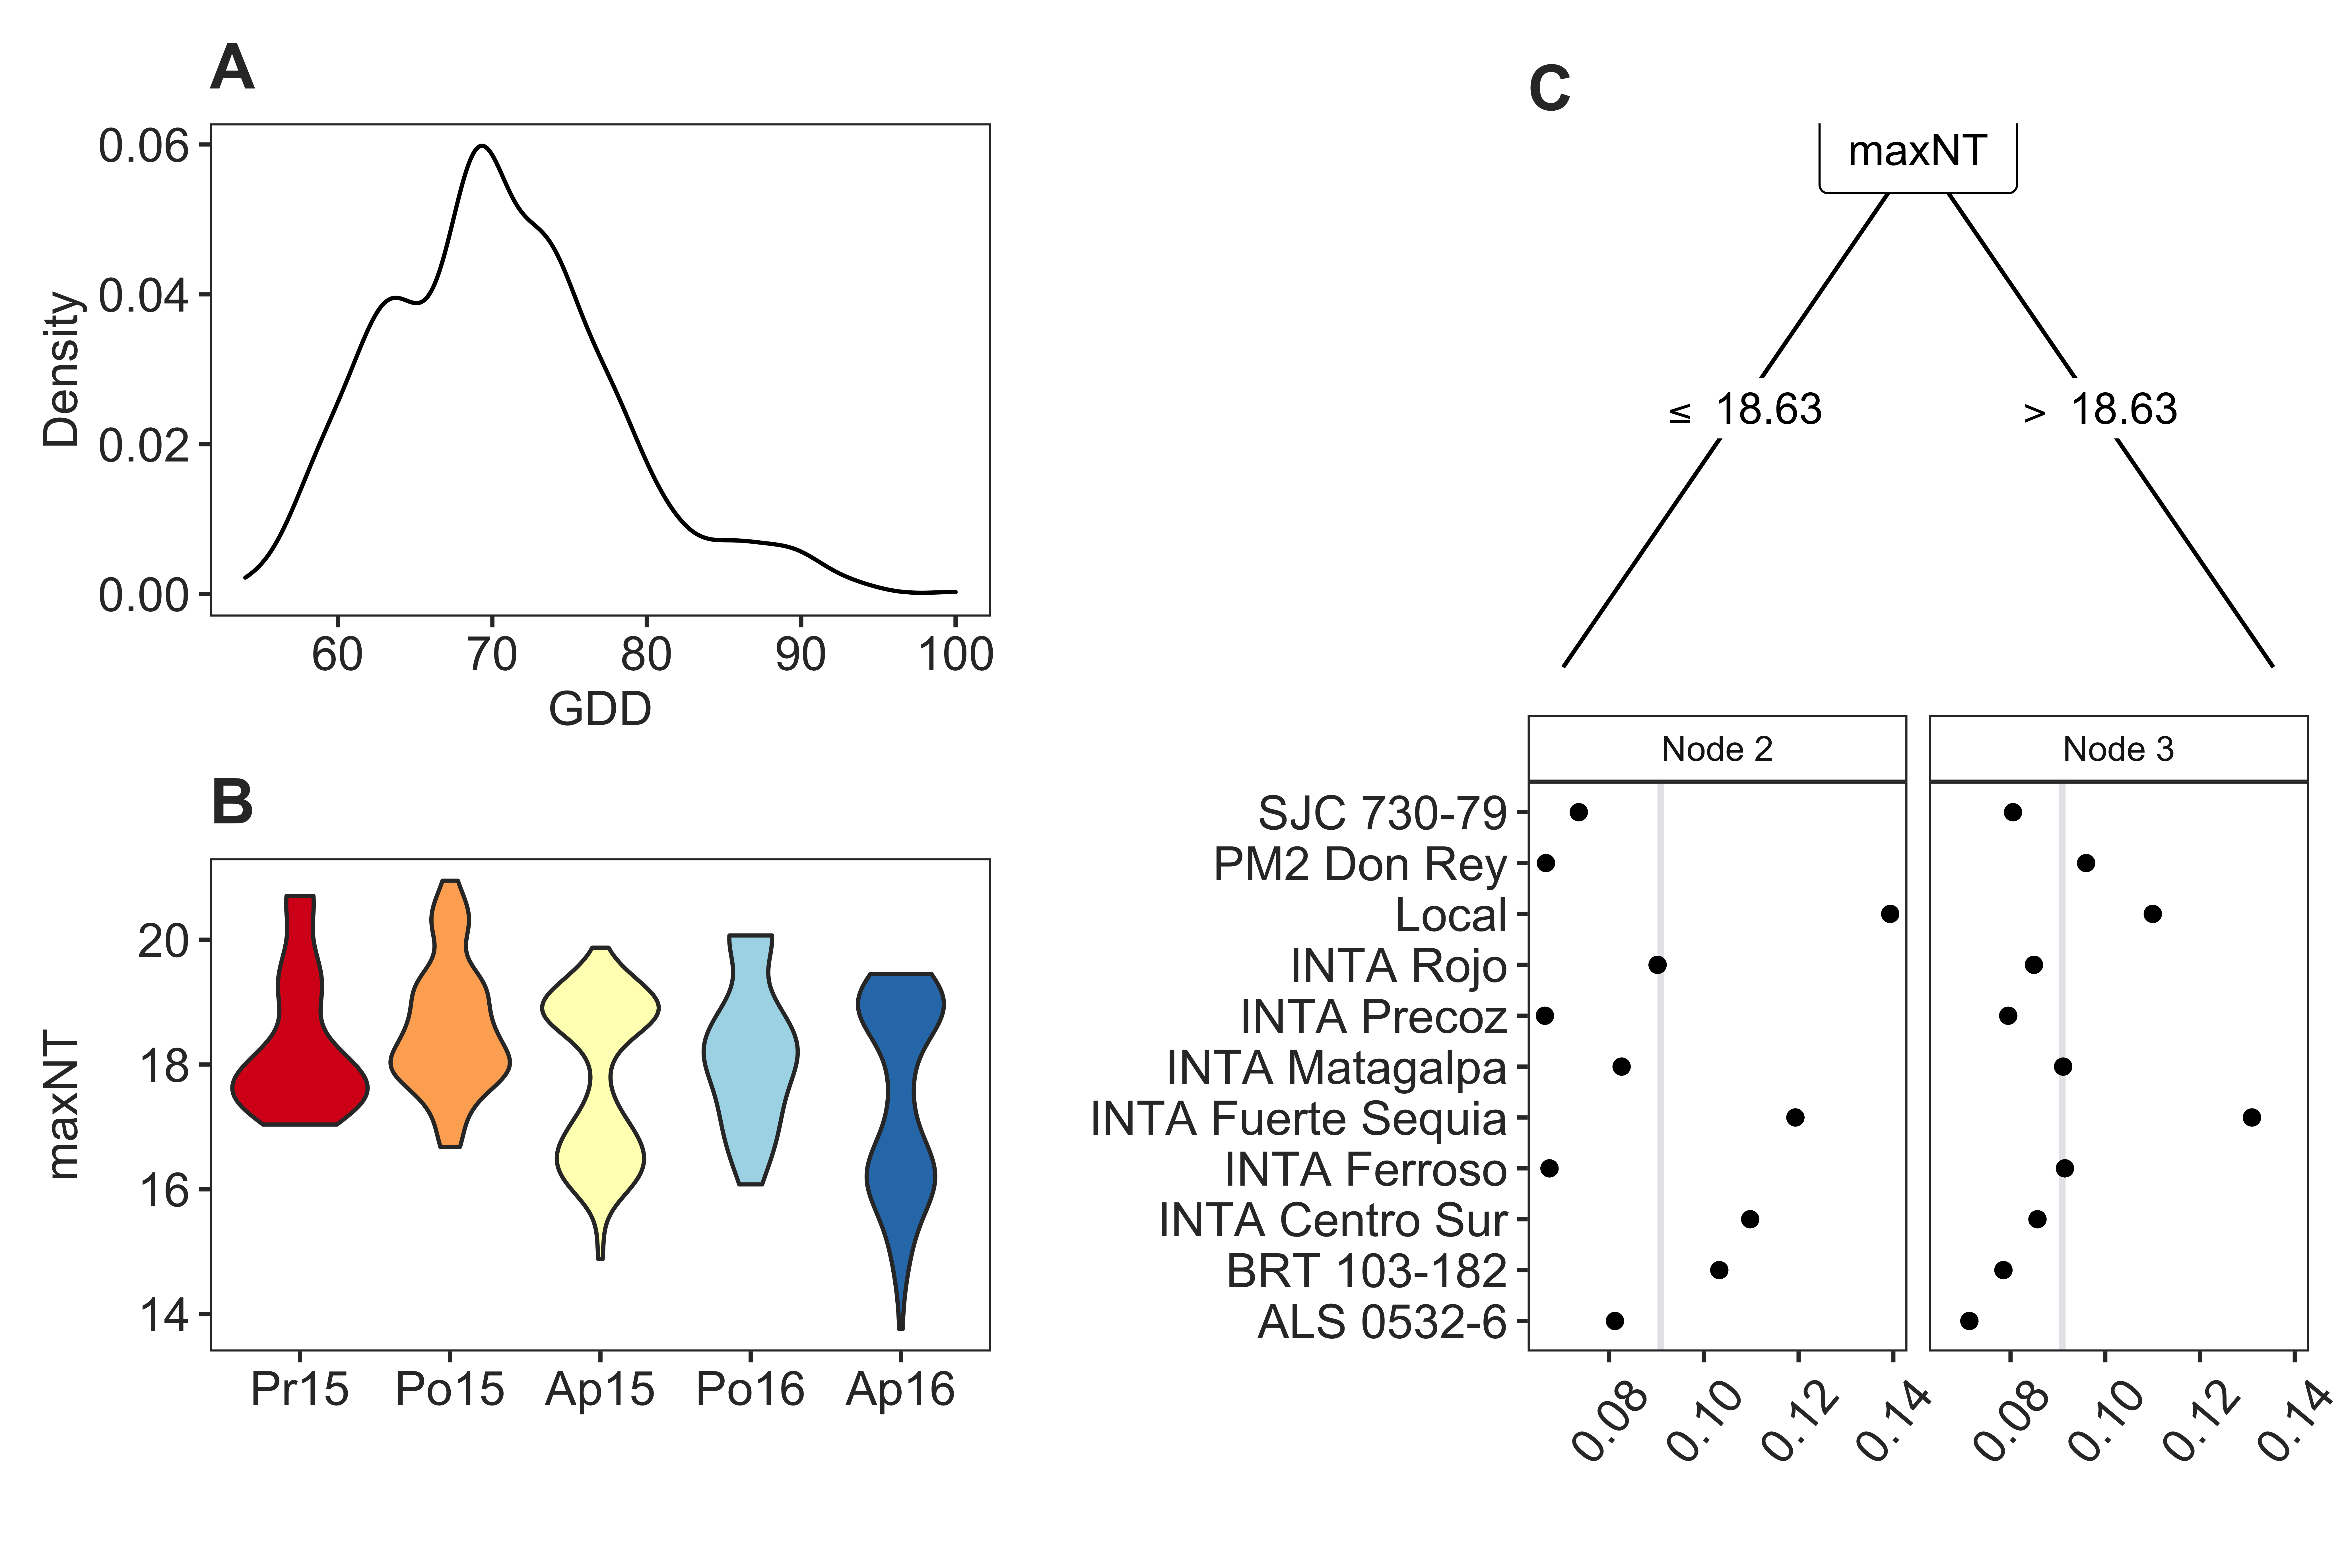
\includegraphics[width=0.8\linewidth]{cbean} \caption{Fig. 1. Application of climatrends functions to support the analysis of a citizen-science data testing 11 common bean varieties in Nicaragua. (A) Days required to reach 900 growing-degree days from planting date calculated using the function GDD(). (B) Maximum night temperature (°C) distributed across seasons computed using the function temperature(). (C) Plackett-Luce Tree showing the probability of one common bean variety has to win against the others (axys X) in three different nodes splitted with the summer days (day temperature > 30 °C) and maximum night temperature (°C). Note: the first season (primera, Pr) spans from May to August, the second (postrera, Po) from September to October, and the third (apante, Ap) from November to January.}\label{fig:fig_cbean}
\end{figure}

\end{document}
